\documentclass[a4paper]{article}

\usepackage[T1]{fontenc}
\usepackage{titling}
\usepackage{amsmath}
\usepackage{amsfonts}
\usepackage{graphicx}
\usepackage{mathtools}
\usepackage[includeheadfoot,margin=1in]{geometry}

\usepackage{chngcntr}
\counterwithin{figure}{section}

\usepackage{caption}
\usepackage{subcaption}

\usepackage{fancyhdr}
\pagestyle{fancy}




\renewcommand{\headrulewidth}{0.5pt}

\numberwithin{equation}{section}
\usepackage[numbered, framed]{matlab-prettifier}

\lstset{
	style              = Matlab-editor,
	escapechar         = ",
	mlshowsectionrules = true,
	tabsize            = 2,
}



\setlength{\droptitle}{-8em}

\title{Sockets assignment}

\author{\textbf{Wojciech Dziwulski, A0153992U}}

\date{}

\begin{document}

\maketitle

\begin{enumerate}
\item Relationship between \textbf{transfer time} and \textbf{packet size} (at constant error probability)

Transfer time is lower as the packet size increases. This is because more time is taken to service all packets separately.

\begin{figure}[h!]
	\centering
	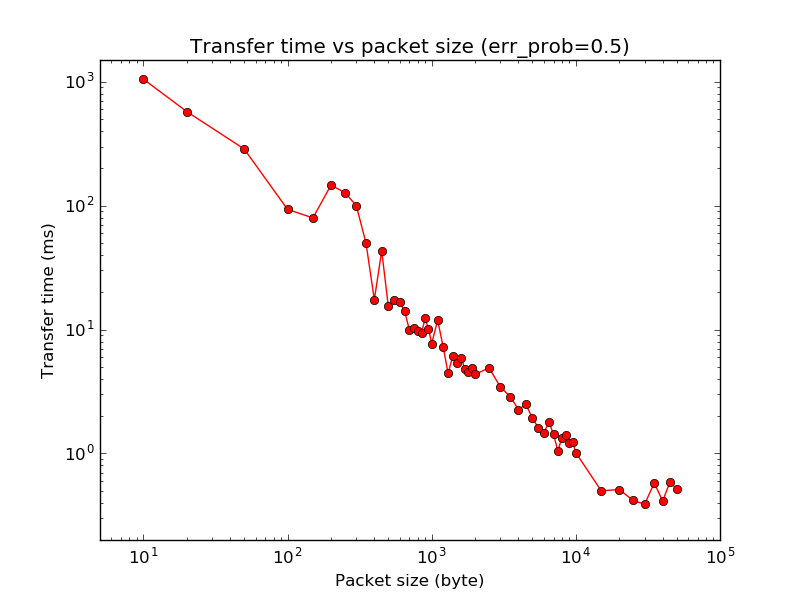
\includegraphics[page=1,width=0.60\textwidth]{Ex4/timeVpacketsize.png}
	\caption{\label{fig:diagram}{Transfer time vs packet size at error probability=50\%}}
\end{figure}

\item Relationship between \textbf{throughput} and \textbf{packet size} (at constant error probability)

Throughput is higher as the packet size increases. This because the transfer time decreases.

\begin{figure}[h!]
	\centering
	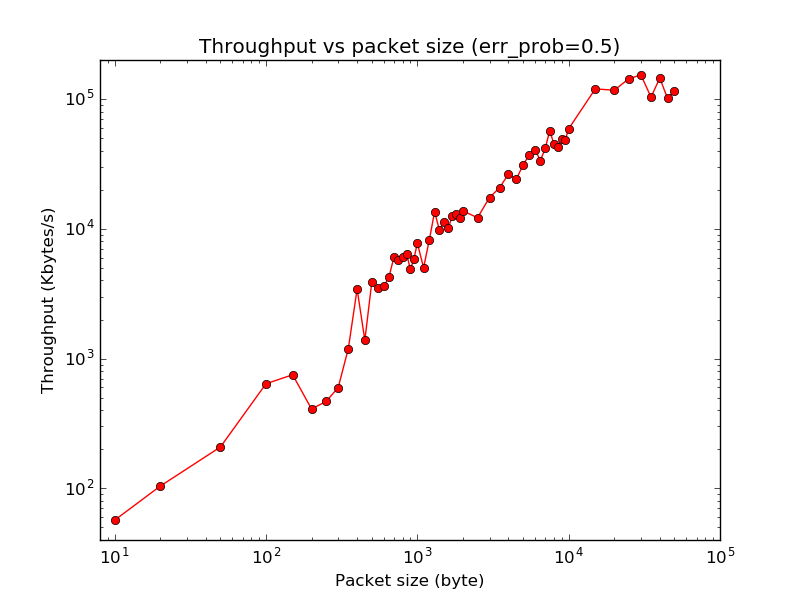
\includegraphics[page=1,width=0.60\textwidth]{Ex4/throughputVpacketsize.png}
	\caption{\label{fig:diagram}{Throughput vs packet size at error probability=50\%}}
\end{figure}

\item Relationship between \textbf{transfer time} and \textbf{error probability} (at constant packet size)

The transfer time increases as the error probability increases. This is because we need to complete more transfers in total.

\begin{figure}[h!]
	\centering
	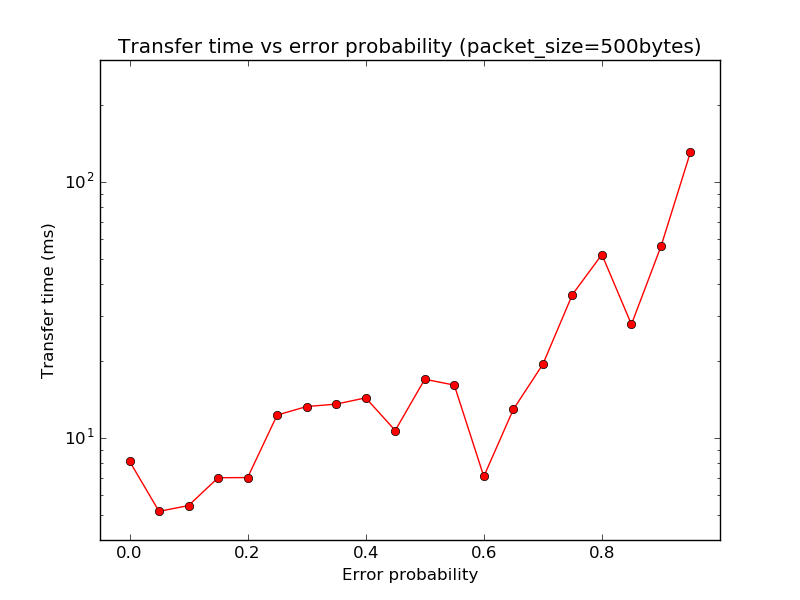
\includegraphics[page=1,width=0.60\textwidth]{Ex4/timeVprobability.png}
	\caption{\label{fig:diagram}{Transfer time vs error probability at packet size = 500 bytes}}
\end{figure}

\item Relationship between \textbf{throughput} and \textbf{error probability} (at constant packet size)

The throughput decreases as the error probability increases. This is because the transfer time increases.

\begin{figure}[h!]
	\centering
	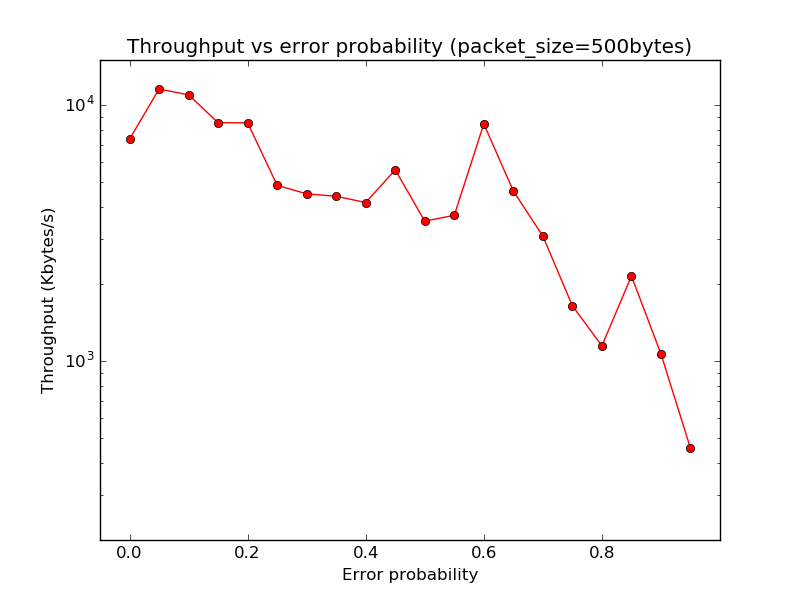
\includegraphics[page=1,width=0.60\textwidth]{Ex4/throughputVprobability.png}
	\caption{\label{fig:diagram}{Throughput vs error probability at packet size = 500 bytes}}
\end{figure}

\end{enumerate}

\end{document}